\documentclass[10pt,a4paper]{article}

% ----- Encodage & langue -----
\usepackage[T1]{fontenc}
\usepackage[utf8]{inputenc}
\usepackage[french]{babel}

% ----- Mise en page -----
\usepackage{geometry}
\geometry{top=1.5cm,bottom=1.5cm,left=1.5cm,right=1.5cm}

% Colonnes
\usepackage{multicol}
\setlength{\columnsep}{0.75cm}            % espace entre colonnes
\setlength{\columnseprule}{0.2pt}      % épaisseur de la ligne
\def\columnseprulecolor{\color{Couleur8}} % couleur de la ligne

% Maths et figures
\usepackage{amsmath, amssymb}
\usepackage{tikz}
\usetikzlibrary{babel,arrows,calc,fit,patterns,plotmarks,shapes.geometric,shapes.misc,shapes.symbols,shapes.arrows,shapes.callouts, shapes.multipart, shapes.gates.logic.US,shapes.gates.logic.IEC, er, automata,backgrounds,chains,topaths,trees,petri,mindmap,matrix, calendar, folding,fadings,through,positioning,scopes,decorations.fractals,decorations.shapes,decorations.text,decorations.pathmorphing,decorations.pathreplacing,decorations.footprints,decorations.markings,shadows}

\usetikzlibrary{calc}
\usepackage{graphicx}
% Listes compactes
\usepackage{enumitem}
\setlist{nosep, itemsep=0.4em, parsep=0pt}
\setlist[enumerate,1]{label=\alph*.}

% Couleurs
\usepackage{xcolor}
\definecolor{exoblue}{HTML}{005F73}

%----------------------------------------------------------------------------------------
%	 COULEURS
%----------------------------------------------------------------------------------------

\definecolor{Couleur1}{HTML}{8b1f30}
\definecolor{Couleur2}{HTML}{725E74}
\definecolor{Couleur3}{HTML}{78985b}
\definecolor{Couleur4}{HTML}{db3e56}
\definecolor{Couleur5}{HTML}{487C4B}
\definecolor{Couleur6}{HTML}{CF6876}
\definecolor{Couleur7}{HTML}{A5C03F} %Vert
\definecolor{Couleur8}{HTML}{D36740} %Orange
\definecolor{Couleur9}{HTML}{7BB48A} %Bleu-Vert
\definecolor{Couleur10}{HTML}{EA8556} %Orange
\definecolor{Couleur11}{HTML}{E6B459} %Jaune
\definecolor{Couleur12}{HTML}{9AC8EB} %Bleu

\definecolor{Bord1}{HTML}{302635}
\definecolor{Bord2}{HTML}{725E74}
\definecolor{Bord3}{HTML}{938999}
\definecolor{Bord4}{HTML}{817888}
\definecolor{Bord5}{HTML}{487C4B}
\definecolor{Bord6}{HTML}{8C436B}
\definecolor{Bord7}{HTML}{A5C03F} %Vert
\definecolor{Bord8}{HTML}{D36740} %Orange

% ----- Police sans serif -----
\renewcommand{\familydefault}{\sfdefault}

% ----- Exercice -----
\newcounter{exo}
\newcommand{\exo}[1][]{%
  \refstepcounter{exo}%
  \textbf{\textcolor{Couleur8}{\\[0.3cm]\theexo.}}%
  \if\relax\detokenize{#1}\relax\else\ \textbf{#1}\fi\ %
}

\newcommand{\ligne}{\noindent\dotfill\vspace{0.6em}}



\begin{document}
\begin{Large}\textbf{\textcolor{Couleur8}{EXERCICES - Chapitre 15 - Proportion}} \end{Large}
\begin{multicols}{2}
%1
\exo \textit{Exprimer des proportions.}

\begin{enumerate}[itemsep=1em]
	\item Dans un sac contenant 38 billes, 17 billes sont orange. \\
Quelle est la proportion de billes orange ? \ligne

	\item Dans une bouteille de 50 cL, il y a 13 cL de sirop. \\
Quelle est la proportion de sirop ?\ligne

	\item Dans une entreprise de 28 salariés, 12 portent des lunettes.\\
Quelle est la proportion de salariés qui ne portent pas de lunettes ?\ligne

	\item Mathieu a ramassé 5 kg de pommes et 9 kg de poires.\\
Quelle est la proportion de pommes ?\ligne

	\item Un match de football est composé de 2 mi-temps de 45 minutes, entrecoupées d'une pause de 10 minutes.\\
Quelle proportion de la durée du match cette pause représente-t-elle ?\ligne

	\item Dans un sac de 43 bonbons, 27 sont rouges, 4 sont verts et les autres sont bleus.\\
Quelle est la proportion de bonbons bleus ?\ligne

\end{enumerate}

\exo Dans la classe de 6°1, il y a 12 filles et 9 garçons. Dans la classe de 6º 4, il y a 16 filles sur un total de 28 élèves. La proportion de filles est-elle la même dans les deux classes ? Explique.

\ligne

\ligne

\ligne

\ligne

\ligne

\exo Le cocktail « Fruit des iles » est composé...
\begin{itemize}
\item de 6 cL de jus de litchi ;
\item de 8 cL de jus de kiwi ;
\item de 12 cL de jus de fruit de la passion ;
\item de 10 cL de jus de goyave.
\end{itemize}
Quelle est la proportion de chaque jus de fruit dans ce cocktail ?

\ligne

\ligne

\ligne

\ligne

\ligne

\columnbreak
\exo Parmi ces boutons, quelle est la proportion ...

\begin{center}
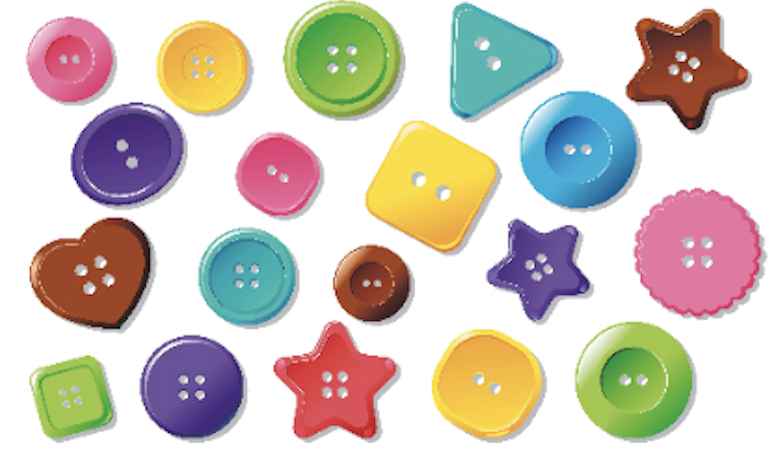
\includegraphics[scale=0.5]{IMG/Boutons.png}
\end{center}

\begin{enumerate}
\item de boutons roses ? \ligne

\item  de boutons à 4 trous ?\ligne

\item  de boutons à 2 trous ?\ligne

\item  de boutons « cœur » ?\ligne

\item  de boutons ronds non dentelés ?\ligne

\end{enumerate}


\exo Dans une compétition de judo, voici le nombre de benjamins qui participent, selon leur catégorie de poids. Complète le tableau, en indiquant la proportion de participants de chaque catégorie.

\begin{center}
\renewcommand{\arraystretch}{2}
\begin{tabular}{|c|c|c|c|c|c|c|c|c|}
\hline
\textbf{Poids en kg} 
& \rotatebox{90}{-30}
& \rotatebox{90}{30 à 34}
& \rotatebox{90}{34 à 38}
& \rotatebox{90}{38 à 42}
& \rotatebox{90}{42 à 46}
& \rotatebox{90}{46 à 50}
& \rotatebox{90}{50 à 55}
& \rotatebox{90}{55 à 60} \\
\hline
\textbf{Nombre} 
& 10 & 25 & 26 & 15 & 13 & 5 & 4 & 2 \\
\hline
\textbf{Proportion} 
&  &  &  &  &  &  &  &  \\
\hline
\end{tabular}
\end{center}

\exo Parmi l'ensemble de ces monstres, quelle la proportion en pourcentage...

\begin{center}
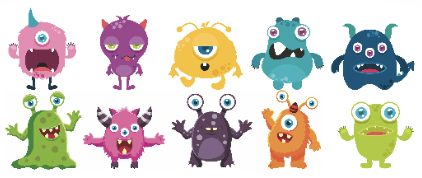
\includegraphics[scale=0.8]{IMG/Monstres.png}
\end{center}
\begin{enumerate}
\item des monstres avec un seul œil ? \ligne

\item des monstres avec deux yeux ? \ligne

\item des monstres avec trois yeux ?\ligne
\end{enumerate}

\exo Quelle est la proportion de voyelles en pourcentage dans chacune des phrases ?

\begin{enumerate}
\item \textit{Patience passe science.}

\ligne


\item \textit{Une heure de conversation vaut mieux que cinquante lettres.}

\ligne

\end{enumerate}
\end{multicols}


\end{document}